
\documentclass[12pt]{article}
\usepackage{amsmath}
\DeclareMathOperator*{\argmin}{arg\,min} % thin space, limits underneath in displays
\DeclareMathOperator*{\argmax}{arg\,max} % thin space, limits underneath in displays
\newtheorem{thm}{Theorem}
\usepackage{amssymb}
\usepackage{amsfonts}
\usepackage{mathrsfs}
\usepackage{bm}
\usepackage{indentfirst}
\setlength{\parindent}{0em}
\usepackage[margin=1in]{geometry}
\usepackage{graphicx}
\usepackage{setspace}
\doublespacing
\usepackage[flushleft]{threeparttable}
\usepackage{booktabs,caption}
\usepackage{float}
\usepackage{graphicx}

\usepackage{import}
\usepackage{xifthen}
\usepackage{pdfpages}
\usepackage{transparent}

\newcommand{\incfig}[1]{%
\def\svgwidth{\columnwidth}
\import{./figures/}{#1.pdf_tex}
}


\usepackage{graphicx}
\usepackage{xspace,color}
\usepackage{url}
\usepackage{listings}


\lstset{commentstyle=\color{gray},keywordstyle=\color{black},
showstringspaces=false, basicstyle = \small
} %% basicstyle set fontsize
\lstnewenvironment{rc}[1][]{\lstset{language=R}}{}
\newcommand{\ri}[1]{\lstinline{#1}}  %% Short for 'R inline'



\lstdefinelanguage{language=R}{
numbers=left,
numberstyle=\footnotesize,
numbersep=1em,
xleftmargin=1em,
framextopmargin=2em,
framexbottommargin=2em,
showspaces=false,
showtabs=false,
showstringspaces=false,
frame=l,
tabsize=4,
}



\title{Linear Regression}
\author{Synferlo}
\date{May, 10}


\begin{document}
\maketitle
\newpage



\section{Simple Linear Regression}

\subsection{Estimation}

\begin{equation*}
 \widehat{y} =  \widehat{\beta_0} +  \widehat{\beta_1} x
\end{equation*}

\begin{equation*}
 \widehat{\beta_1} = \rho_{xy} \frac{s_{y}}{s_{x}},
 \text{ and }  \widehat{\beta_0} =  \overline{y} -  \widehat{\beta_1}
   \overline{x}
\end{equation*}

$  \overline{x},  \overline{y} $: sample means\\
$ s_{x}, s_{y} $: sample standard deviation\\
$ \rho_{xy} $: the estimate of correlation between $ X $ and $ Y $
based on the data.\\



\subsection{Statistical Inference}

\begin{table}[h!]
\begin{center}
	
\begin{threeparttable}
		\caption{Price and Volume (unnormalized result)}			

\begin{tabular}{lllll}
\\ [-1.8ex]
\hline
\hline \\[-1.8ex]
 & {\textbf {Coefs}} & {\textbf {SE}} & {\textbf {t-value}} & 
 {\textbf {p-value}}\\
\\ [-1.8ex]
\hline \\[-1.8ex]

 (Intercept) &2.342e+03  &8.799e+01   &26.62   &$<2e-16$ ***\\
 Volume      &2.696e-07  &5.252e-09   &51.33   &$<2e-16$ ***\\
\hline \\[-1.8ex]
Multiple R-squared:  &0.5061 &Adjusted R-squared:  &0.506\\
\\ [-1.8ex]
\hline \\[-1.8ex]

\end{tabular}
\begin{tablenotes}
\small
\item Signif. codes:  0 ‘***’ 0.001 ‘**’ 0.01 ‘*’ 0.05 ‘.’ 0.1 ‘ ’ 1\\
\item Residual standard error: 3803 on 2571 degrees of freedom\\
\item F-statistic:  2635 on 1 and 2571 DF,  p-value: $< 2.2e-16$\\
\end{tablenotes}


\end{threeparttable}
\end{center}
\end{table}



$ p $-value and $ t $-value for the coefs are the results of a two-
tailed test based on $ t $-distribution with DOF = 2.
\begin{align*}
H_0:& \beta_{j} = 0\\
H_1:& \beta_{j} \ne 0
\end{align*}

where $ j = 0 $ for the intercept $ \beta_0 $, and $ j = 1 $ for the
coef. of the volume.




\subsubsection{$ R^{2} $ and adjusted $ R^{2} $}

\begin{equation*}
R^{2} = \rho_{xy}^{2}
\end{equation*}

In R, 
\begin{rc}
# compute correlation then square it.
cor(df$Open_price, df$Volume, use = 'complete.obs')**2
# [1] 0.5061467
\end{rc}


You can check this 0.506 with the R-squared we've got from 
$ summary(result) $. They are exactly the same.



R-squared tells us 50 percent of the variation in the price can be 
attributed to volume.\\

The adjusted R-squared is important {\underline {ONLY IF}} you are
using the coef of determination to assess the overall quality of the
fitted model in terms of a balance between goodness of fit(GOF) and
complexity.



\subsubsection{Other summary output}
Residual standard error is the estimated SE of the $ \varepsilon $,
i.e., $  \widehat{\sigma} $.





\subsection{Categorical Predictor}

Explanatory variables can be categorical.

\subsubsection{Binary Variables}

\begin{equation*}
Y = \beta_0 + \beta_1 X + \varepsilon
\end{equation*}
X can be either 0 or 1.

If so, the interpretation of $ \beta $ would be different.
It's better to think of them like two {\underline {intercepts}},
where $ \beta_0 $ provides the {\underline {baseline}} of the response
when $ X = 0 $, and $ \beta_1 $ represents the {\underline {additive
effect}} on the mean response if $ X = 1 $.




\subsubsection{Multilevel variables}
The categorical variables have more than two levels.
For example, there can be many levels under education, e.g., 
high school, college, master, phd, etc.

Suppose there are $ k $ levels, then variable X can be written as
\begin{align*}
X &= 1,2,3,...,k\\
X_{(1)} = 0,1 \quad X_{(2)} &= 0,1 \quad ... X_{(k)} = 0,1
\end{align*}

And we can write the model,
\begin{equation*}
 \widehat{y} =  \widehat{\beta}_{0} +  \widehat{\beta}_{1}X_{(2)}
  +  \widehat{\beta}_{(2)}X_{(3)} + ... +  \widehat{\beta}_{k - 1}X_{(k)}
\end{equation*}

We normally use $ k - 1 $ of the dummy variables. Also,
each observation only satisfy one of the levels, i.e., if you are a
Ph.D. student, then you cannot be a high school student.
Hence, when $ X_{(i)} = 1 $, all others equals to zero.

So, if one observation belongs to level 3, then the model (
the predicted mean) would be
\begin{equation*}
 \widehat{y} =  \widehat{\beta}_{0} +  \widehat{\beta}2
\end{equation*}

Since the reference level(that omitted dummy) is defined as 1, 
if an observation has values of zero for all other dummies, it
implies the obs originally had X = 1.
\begin{equation*}
 \widehat{y} =   \widehat{\beta}_{0}
\end{equation*}
Here we have the result of a model with a dummy has four levels (
Heavy, Never, Occas, Regular), where Heavy is the reference.

\begin{figure}[H]
		\center{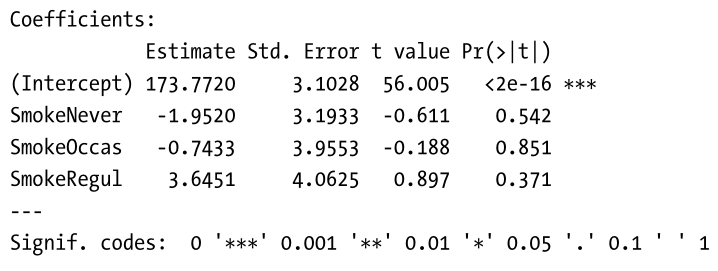
\includegraphics[scale =.7 ]  {figures/dummies_in_linear_model.png}}
\end{figure}



The observation in the reference category Heavy is represented solely
by $  \widehat{\beta}_{0} = 173.7720 $.



















\end{document}

